\documentclass[a4paper]{article}
\usepackage[a4paper, margin=1in]{geometry}
% Some basic packages
\usepackage[utf8]{inputenc}
\usepackage[T1]{fontenc}
\usepackage{textcomp}
\usepackage[dutch]{babel}
\usepackage{url}
\usepackage{graphicx}
\usepackage{float}
\usepackage{booktabs}
\usepackage{enumitem}

\pdfminorversion=7

% Don't indent paragraphs, leave some space between them
\usepackage{parskip}

% Hide page number when page is empty
\usepackage{emptypage}
\usepackage{subcaption}
\usepackage{multicol}
\usepackage{xcolor}

% Other font I sometimes use.
% \usepackage{cmbright}

% Math stuff
\usepackage{amsmath, amsfonts, mathtools, amsthm, amssymb}
% Fancy script capitals
\usepackage{mathrsfs}
\usepackage{cancel}
% Bold math
\usepackage{bm}
% Some shortcuts
\newcommand\N{\ensuremath{\mathbb{N}}}
\newcommand\R{\ensuremath{\mathbb{R}}}
\newcommand\Z{\ensuremath{\mathbb{Z}}}
\renewcommand\O{\ensuremath{\emptyset}}
\newcommand\Q{\ensuremath{\mathbb{Q}}}
\newcommand\C{\ensuremath{\mathbb{C}}}

% Easily typeset systems of equations (French package)
\usepackage{systeme}

% Put x \to \infty below \lim
\let\svlim\lim\def\lim{\svlim\limits}

%Make implies and impliedby shorter
\let\implies\Rightarrow
\let\impliedby\Leftarrow
\let\iff\Leftrightarrow
\let\epsilon\varepsilon

% Add \contra symbol to denote contradiction
\usepackage{stmaryrd} % for \lightning
\newcommand\contra{\scalebox{1.5}{$\lightning$}}

% \let\phi\varphi

% Command for short corrections
% Usage: 1+1=\correct{3}{2}

\definecolor{correct}{HTML}{009900}
\newcommand\correct[2]{\ensuremath{\:}{\color{red}{#1}}\ensuremath{\to }{\color{correct}{#2}}\ensuremath{\:}}
\newcommand\green[1]{{\color{correct}{#1}}}

% horizontal rule
\newcommand\hr{
    \noindent\rule[0.5ex]{\linewidth}{0.5pt}
}

% hide parts
\newcommand\hide[1]{}

% si unitx
\usepackage{siunitx}
\sisetup{locale = FR}

% Environments
\makeatother
% For box around Definition, Theorem, \ldots
\usepackage{mdframed}
\mdfsetup{skipabove=1em,skipbelow=0em}
\theoremstyle{definition}
\newmdtheoremenv[nobreak=true]{definitie}{Definitie}
\newmdtheoremenv[nobreak=true]{eigenschap}{Eigenschap}
\newmdtheoremenv[nobreak=true]{gevolg}{Gevolg}
\newmdtheoremenv[nobreak=true]{lemma}{Lemma}
\newmdtheoremenv[nobreak=true]{propositie}{Propositie}
\newmdtheoremenv[nobreak=true]{stelling}{Stelling}
\newmdtheoremenv[nobreak=true]{wet}{Wet}
\newmdtheoremenv[nobreak=true]{postulaat}{Postulaat}
\newmdtheoremenv{conclusie}{Conclusie}
\newmdtheoremenv{toemaatje}{Toemaatje}
\newmdtheoremenv{vermoeden}{Vermoeden}
\newtheorem*{herhaling}{Herhaling}
\newtheorem*{intermezzo}{Intermezzo}
\newtheorem*{notatie}{Notatie}
\newtheorem*{observatie}{Observatie}
\newtheorem*{oef}{Oefening}
\newtheorem*{opmerking}{Opmerking}
\newtheorem*{praktisch}{Praktisch}
\newtheorem*{probleem}{Probleem}
\newtheorem*{terminologie}{Terminologie}
\newtheorem*{toepassing}{Toepassing}
\newtheorem*{uovt}{UOVT}
\newtheorem*{vb}{Voorbeeld}
\newtheorem*{vraag}{Vraag}

\newmdtheoremenv[nobreak=true]{definition}{Definition}
\newtheorem*{eg}{Example}
\newtheorem*{notation}{Notation}
\newtheorem*{previouslyseen}{As previously seen}
\newtheorem*{remark}{Remark}
\newtheorem*{note}{Note}
\newtheorem*{problem}{Problem}
\newtheorem*{observe}{Observe}
\newtheorem*{property}{Property}
\newtheorem*{intuition}{Intuition}
\newmdtheoremenv[nobreak=true]{prop}{Proposition}
\newmdtheoremenv[nobreak=true]{theorem}{Theorem}
\newmdtheoremenv[nobreak=true]{corollary}{Corollary}

% End example and intermezzo environments with a small diamond (just like proof
% environments end with a small square)
\usepackage{etoolbox}
\AtEndEnvironment{vb}{\null\hfill$\diamond$}%
\AtEndEnvironment{intermezzo}{\null\hfill$\diamond$}%
% \AtEndEnvironment{opmerking}{\null\hfill$\diamond$}%

% Fix some spacing
% http://tex.stackexchange.com/questions/22119/how-can-i-change-the-spacing-before-theorems-with-amsthm
\makeatletter
\def\thm@space@setup{%
  \thm@preskip=\parskip \thm@postskip=0pt
}


% Exercise 
% Usage:
% \oefening{5}
% \suboefening{1}
% \suboefening{2}
% \suboefening{3}
% gives
% Oefening 5
%   Oefening 5.1
%   Oefening 5.2
%   Oefening 5.3
\newcommand{\oefening}[1]{%
    \def\@oefening{#1}%
    \subsection*{Oefening #1}
}

\newcommand{\suboefening}[1]{%
    \subsubsection*{Oefening \@oefening.#1}
}


% \lecture starts a new lecture (les in dutch)
%
% Usage:
% \lecture{1}{di 12 feb 2019 16:00}{Inleiding}
%
% This adds a section heading with the number / title of the lecture and a
% margin paragraph with the date.

% I use \dateparts here to hide the year (2019). This way, I can easily parse
% the date of each lecture unambiguously while still having a human-friendly
% short format printed to the pdf.

\usepackage{xifthen}
\def\testdateparts#1{\dateparts#1\relax}
\def\dateparts#1 #2 #3 #4 #5\relax{
    \marginpar{\small\textsf{\mbox{#1 #2 #3 #5}}}
}

\def\@lecture{}%
\newcommand{\lecture}[3]{
    \ifthenelse{\isempty{#3}}{%
        \def\@lecture{Lecture #1}%
    }{%
        \def\@lecture{Lecture #1: #3}%
    }%
    \subsection*{\@lecture}
    \marginpar{\small\textsf{\mbox{#2}}}
}



% These are the fancy headers
\usepackage{fancyhdr}
\pagestyle{fancy}

% LE: left even
% RO: right odd
% CE, CO: center even, center odd
% My name for when I print my lecture notes to use for an open book exam.
% \fancyhead[LE,RO]{Gilles Castel}

\fancyhead[RO,LE]{\@lecture} % Right odd,  Left even
\fancyhead[RE,LO]{}          % Right even, Left odd

\fancyfoot[RO,LE]{\thepage}  % Right odd,  Left even
\fancyfoot[RE,LO]{}          % Right even, Left odd
\fancyfoot[C]{\leftmark}     % Center

\makeatother




% Todonotes and inline notes in fancy boxes
\usepackage{todonotes}
\usepackage{tcolorbox}

% Make boxes breakable
\tcbuselibrary{breakable}

% Verbetering is correction in Dutch
% Usage: 
% \begin{verbetering}
%     Lorem ipsum dolor sit amet, consetetur sadipscing elitr, sed diam nonumy eirmod
%     tempor invidunt ut labore et dolore magna aliquyam erat, sed diam voluptua. At
%     vero eos et accusam et justo duo dolores et ea rebum. Stet clita kasd gubergren,
%     no sea takimata sanctus est Lorem ipsum dolor sit amet.
% \end{verbetering}
\newenvironment{verbetering}{\begin{tcolorbox}[
    arc=0mm,
    colback=white,
    colframe=green!60!black,
    title=Opmerking,
    fonttitle=\sffamily,
    breakable
]}{\end{tcolorbox}}

% Noot is note in Dutch. Same as 'verbetering' but color of box is different
\newenvironment{noot}[1]{\begin{tcolorbox}[
    arc=0mm,
    colback=white,
    colframe=white!60!black,
    title=#1,
    fonttitle=\sffamily,
    breakable
]}{\end{tcolorbox}}




% Figure support as explained in my blog post.
\usepackage{import}
\usepackage{xifthen}
\usepackage{pdfpages}
\usepackage{transparent}
\newcommand{\incfig}[1]{%
    \def\svgwidth{\columnwidth}
    \import{./figures/}{#1.pdf_tex}
}

% Fix some stuff
% %http://tex.stackexchange.com/questions/76273/multiple-pdfs-with-page-group-included-in-a-single-page-warning
\pdfsuppresswarningpagegroup=1

\title{\Huge{Probability I}\\ Proof of Ergodic Theorem}
\author{\huge{Daniel Yu}}
\date{October 31, 2024}

\pdfsuppresswarningpagegroup=1

\begin{document}
\maketitle
\newpage% or \cleardoublepage
% \pdfbookmark[<level>]{<title>}{<dest>}
\tableofcontents
\pagebreak

\section{Proof of Ergodic Theorem}
\begin{note}
    The ergodic theorem for finite state markov chain states the following. Let $P$ be a the transition matrix. Then $\lim_{n \to \infty}$ exists has constant columns and each row is made up of the unique stationary vectors of $P$. Furthermore, for any intial probability distribution $v$,  $\lim_{n \to \infty} P^{n} v = \pi $ the unique stationary distribution\\ 
\end{note}
\begin{proof}
  $\forall i,j \in \Omega$, if  $x_n$ is irreducible, aperiodic, markov chain, 
   \[
     \lim_{n \to \infty} P[X_n = j \mid X_0 = i] = \pi_j
  .\] 
  where $\pi$ is the stationary distribution vector. If $x_0 \sim \pi$ i.e. $P[x_0 = j] = \pi_j$. What is the distribution of the following?
  \begin{align*}
    P[X_1=k] &= \sum_{j \in \Omega} P[X_1 = k \mid X_0 = j] P[X_0 = j] \\
    &= \sum_{j \in \Omega} P_{j,k} \pi \\
    &= \left( \pi P \right)_{k} \cdot \pi_k 
  .\end{align*}
  If the intial distribution is $\pi$ then the distribution at all times is also $\pi$. Let's consider if $v \neq \pi$. \\

  
  Let $(X_n, Y_n)$ be two pariticles evolving with the same markov chain dynamics (i.e. same transition matrix) where  $X_0 = i$ and $Y_0 \sim \pi$. So $X_n$ evolves in a complicated way but  $Y_n \sim \pi$. At any time $n$, every state  $i$ chooses another state  $k$ with probability  $P_{i,k}$, every particle that was at state $i$ at times  $n$ moves to state  $k$ at time  $n+1$ since the transition probability is the same for $X_n$ and  $Y_n$. This is known as a \textbf{coalescing walk}, when the two particles meet, they now have the same distribution at any time $n+1 $ after.\\


  Let  $T = \min \{n: X_n = Y_n\} $ at any time after $T, X_n = Y_n$ since they follow the same set of instructions.Let's compute,
   \[
     P[X_n = j \mid  X_0 = i, T \leq n] = P[Y_n = j \mid  X_0 = i, T \leq n] = \pi_j
  .\] 
  By law of total probability:
  \begin{align*}
    P[X_n = j \mid  X_0 = i] &= P[X_n = j \mid  n < T, x_0 = i] \cdot P[n < T \mid X_0 = i] + \\
                             &P[X_n = j \mid n \geq T, X_0 = i] \cdot (1-P[n < T \mid X_0 =i ])\\
                             &= P[X_n = j \mid  n < T, X_0 = i] P[n < T \mid  X_0 =i ] + \pi_j ( 1- P[n < T \mid  X_0 = i])\\
                             &= \pi_j + P[n < T \mid X_0 = i] (P[X_n = j \mid n < T, X_0 = i] -\pi_j) \\
    P[X_n = j \mid X_0 =i] - \pi_j &= P[n < T \mid X_0 = i] (P[X_n = j \mid n < T, X_0 = i] -\pi_j) \\
    \| P[X_n = j \mid X_0 = i] - \pi_j \|  &= P[n < T \mid X_0 = i] \| (P[X_n = j \mid n < T, X_0 = i] -\pi_j) \|  \\
                                               &\leq P[n < T \mid X_0=i] \\
   .\end{align*}
    We want to show that $P[n < T \mid X_0 = i] \to 0 $ as $n \to \infty$ since this implies that  $P[X_n = j \mid X_0=i] = \pi_j$ and the random variable $X_n$ approaches the stationary distribution despite the intial distribution. \\


    Consider the $\mid \Omega \mid  \times \mid \Omega \mid $  joint state space $(X_n ,Y_n)$ that describes the markov chain dynamics of $X_n, Y_n$ where
    \[
      (i,j) = \left( X_n, Y_n \right) 
    .\]
    Since $P$ is irreducible and aperiodic, then we can reach any pair  $(i,j)$ from any other state  $(k,l)$. This means that  $P[\text{ everything absorbed eventually}] = 1$. Equivalently, $P[T < \infty] = 1$ and 
     \[
       \lim_{n \to \infty} P[n < T] = P[T= \infty] = 0
    .\] 
    and we conclude that $ \|P[X_n = j\mid  X_0 =i\| \to 0$ as $n \to \infty$. In fact,  $\exists p > 0$ that $P[n < T] = P[n < T] \leq (1-p)^{n}$.
  \end{proof}

\section{Mixing Times}
\begin{note}
  How can we compare distributions? We know that eventually the distirbution will converge to $\pi$ but what is the distribution at $n=100$, what about  $n=1000$? It will be almost  $\pi$ but not quite. 
\end{note}
\begin{definition}
  Let $\Omega$ be finite, and  $u,v$ be two rwo vectors. WE can denote the \textbf{variation distance} as
  \[
  d_{t v} (u, v) = \frac{1}{2} \sum_{i \in \Omega} \|u_i - v_i\|
  .\] 
\end{definition}
Consider the following example:

\begin{figure}[h]
  \centering
  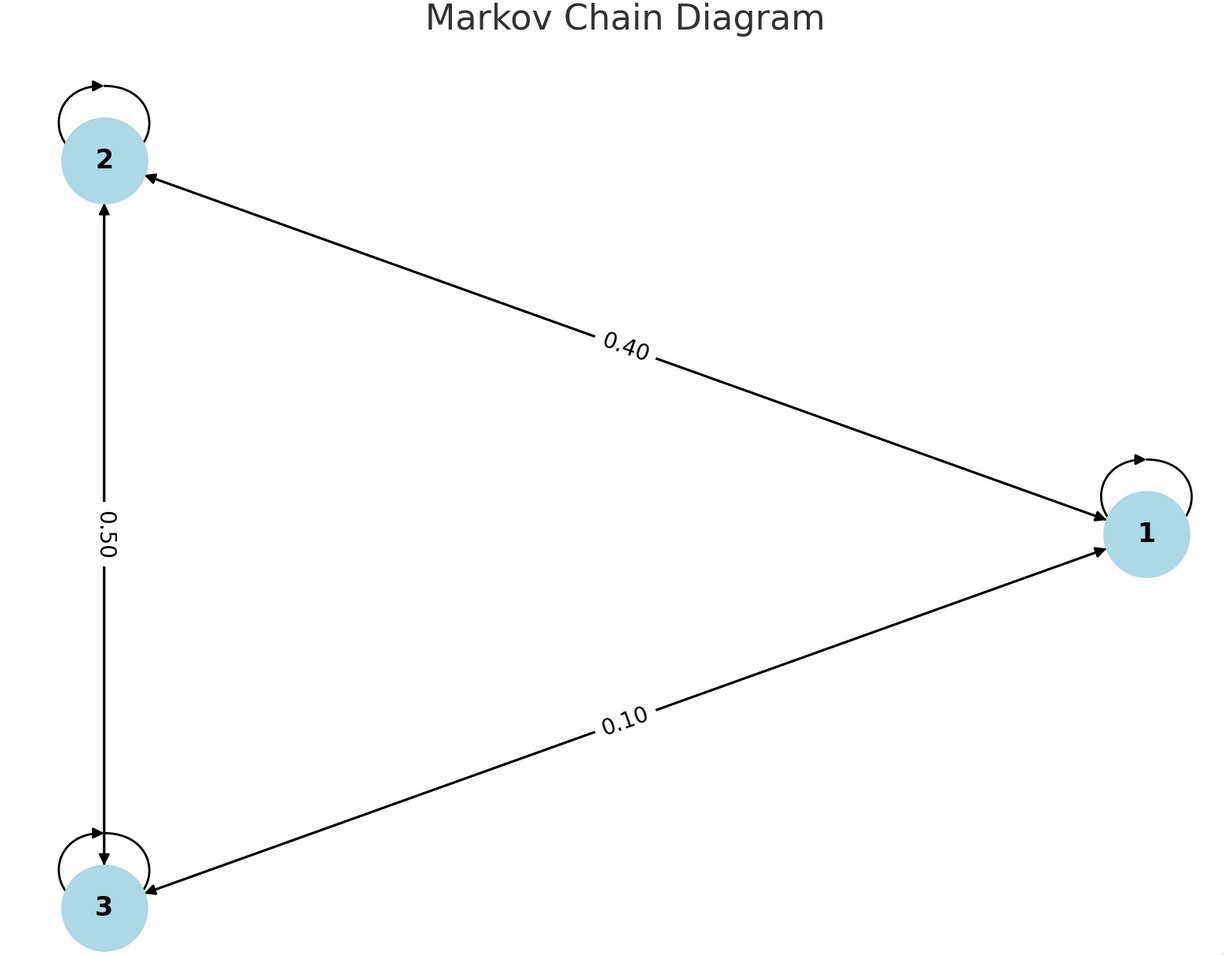
\includegraphics[width=0.8\textwidth]{assets/3_state_markov_chain.png}
  \label{fig:3_state_markov_chain}
\end{figure}
The transition matrix $P$ is \[
P = \begin{bmatrix} 
0.5 & 0.3 & 0.2 \\
0.4 & 0.4 & 0.2 \\
0.1 & 0.5 & 0.4 
\end{bmatrix}, \quad \pi^{(0)} = \begin{bmatrix} 1 \\ 0 \\ 0 \end{bmatrix}
\] Lets consider some intial vector $v= \begin{bmatrix} 1 \\ 0 \\ 0 \end{bmatrix}$
We can compute the variation distance after two steps (how far our distribution $v$ is from the stationary distribution) as follows.
\begin{enumerate}
  \item Solve for $\pi P = \pi$, we get \[
\pi = \begin{bmatrix} 0.267 \\ 0.4 \\ 0.333 \end{bmatrix}
\]
\item Compute $P^{2}$ and $vP^{2} =v^{2}$. \[
P^2 = P \times P = \begin{bmatrix} 
0.5 & 0.3 & 0.2 \\
0.4 & 0.4 & 0.2 \\
0.1 & 0.5 & 0.4 
\end{bmatrix} \times \begin{bmatrix} 
0.5 & 0.3 & 0.2 \\
0.4 & 0.4 & 0.2 \\
0.1 & 0.5 & 0.4 
\end{bmatrix} = \begin{bmatrix} 
0.39 & 0.37 & 0.24 \\
0.38 & 0.38 & 0.24 \\
0.29 & 0.43 & 0.28 
\end{bmatrix}
\], so we get $v^{2} = vP^{2} = \begin{bmatrix} 0.39 & 0.37 & 0.24 \end{bmatrix}$
\item We get that \[
d_{tv}(v^{2}, \pi) = \frac{1}{2} \sum_{i=1}^3 \left| v_i^{(2)} - \pi_i \right| = \frac{1}{2} \left( |0.39 - 0.267| + |0.37 - 0.4| + |0.24 - 0.333| \right) = 0.123
\]

Thus, the total variation distance after 2 steps is approximately \( 0.123 \).
\end{enumerate}

\begin{definition}
  Define $DTM(n) = \text{ distance to mixing time at n} = \sup_{i} d_{t v} (v^{i}_n, \pi)$. If $v_n$ is the distribution of  $v_n$ with any intial conditions,  $d_{t v} (v_n, \pi) \leq DTM(n)$. \\


  We define the mixing time with threshold $\epsilon$ as 
  \[
    \min \{n \mid DTM(n) \leq \epsilon \} 
  .\] 
  i.e. the minimum number of steps to get  $\epsilon$ close to the stationary distribution  $\pi$. The markov chain after this timestep is consider \textbf{mixed}
\end{definition}

Let's continue our previous example. What is the mixing time with $\epsilon = .1$?
\begin{align*}
\text{Step 0:} & \quad v^{(0)} = \begin{bmatrix} 1 & 0 & 0 \end{bmatrix} \\
& \quad d_\text{TV}(v^{(0)}, \pi) = \frac{1}{2} \sum_{i=1}^3 \left| \pi_i^{(0)} - \pi_i \right| = 0.733 \\
\\
\text{Step 1:} & \quad v^{(1)} = v^{(0)} P = \begin{bmatrix} 0.5 & 0.3 & 0.2 \end{bmatrix} \\
& \quad d_\text{TV}(v^{(1)}, \pi) = 0.233 \\
\\
\text{Step 2:} & \quad v^{(2)} = v^{(1)} P = \begin{bmatrix} 0.39 & 0.37 & 0.24 \end{bmatrix} \\
& \quad d_\text{TV}(v^{(2)}, \pi) = 0.123 \\
\\
\text{Step 3:} & \quad v^{(3)} = v^{(2)} P = \begin{bmatrix} 0.35 & 0.39 & 0.26 \end{bmatrix} \\
& \quad d_\text{TV}(v^{(3)}, \pi) = 0.1 \\
\\
\text{Step 4:} & \quad v^{(4)} = \pi^{(3)} P = \begin{bmatrix} 0.33 & 0.4 & 0.27 \end{bmatrix} \\
& \quad d_\text{TV}(v^{(4)}, \pi) = 0.0953
\end{align*}
Thus, the mixing time is $4$.

\begin{theorem}{Perron-Frobenius Theorem}\\
  If $P$ is the transition matrix of an irreducible markov chain then $\lambda=1$ is always an eigenvalue with row-eigenvalue  $\pi$ of strictly positive entries. All other eigenvalues $\{\lambda_{i}\}^{n}_{i=2} $ have $\mid \lambda \mid  < 1$. If $\alpha$ is a row eigenvector of  $P$ with eigenvalue  $\neq 1$, then  $\sum_{i=1}^{n} \alpha_i = 0$.  
\end{theorem}

\begin{note}
  Eigenvalues can be complex. 
\end{note}

\begin{corollary}
  Any vector $P$ with  $p_i \geq 0$ and  $\sum_{i=1}^{n} P_i = 1$ can be written as $P= \pi + \sum_{i=1}^{n} c_i \vec{\alpha_i}$ hwere $c_i \in \R$ and $\alpha_i$ are row vectors of  $P$ with eigenvalue  $\neq 1$.
\end{corollary}

\section{Card Shuffling}
Consider the $n$ card deck is shuffled by moving the top card to a uniformly chosen random position.  $\Omega =$ arrangement of  $n$ cards. Clearly,  $\mid \Omega \mid  = n!$. Every row of $P_{\mid \Omega \mid  \times \mid \Omega \mid}$ would have $n$ positive entries, with probability to be $\frac{1}{n}$ and all entries $0$. It will be a very sparse matrix. \\


It turns out that this matrix is doubly stochastic! The stationary distribution is just the uniform distribution. By the ergodic theorem, this deck is well-shuffled, because  $n \to \infty, \piP^{n} = \pi$ where $\pi$ is the uniform distribution. 

\end{document}
